\section{Design Thinking - 1. Draft}
\emph{How and why did we use Design Thinking?}

\begin{itemize}
    \item Detailed interview methodology: How you recruited participants (social media, personal, etc.), interview duration, recording of interviews, location, incentives offered
    \item Participant demographics: Age ranges, study programs, habits, tech usage patterns
    \item Critical reflection: Honest assessment of design thinking's limitations in your project
    \item Process challenges: What didn't work as expected and how you adapted
\end{itemize}

1. Unsere Projektidee

Mit unserer App möchten wir alleinerziehende Eltern unterstützen, die hauptsächlich für die Betreuung eines Kindes verantwortlich sind. Im Alltag kann es immer wieder passieren, dass Eltern plötzlich verhindert sind. Vielleicht müssen sie unerwartet ins Krankenhaus, haben einen dringenden Termin oder können ihr Kind aus einem anderen Grund nicht rechtzeitig abholen. Besonders für Alleinerziehende kann das schwierig werden, wenn keine zweite Betreuungsperson zur Verfügung steht.

Unsere Idee ist deshalb eine App, mit der Eltern schon im Voraus einen kleinen Kreis aus vertrauten Personen zusammenstellen können. Das könnten zum Beispiel Familienmitglieder, Freunde oder Nachbarn sein. Wenn sie keine Möglichkeit haben geben wir auch die Option  zur Betreuungsagentur yu bitten. Falls kurzfristig Hilfe benötigt wird, sollen diese Personen möglichst schnell informiert werden.

Außerdem können Eltern wichtige Informationen über die Betreuung ihres Kindes hinterlegen, damit die helfende Person weiß, worauf sie achten muss.

Unser Ziel ist es, die Zusammenarbeit zwischen Menschen zu erleichtern, die sich bereits kennen und gegenseitig vertrauen. Im Mittelpunkt stehen dabei drei Dinge: Vertrauen, Sicherheit und gegenseitige Unterstützung.

% ***************************************************************
%           User Persona
% ***************************************************************
\subsection{User Persona}
\emph{Include Activity of Persona.}

Follow the template provided or from the internet to include a visual persona with picture, demographics, goals, frustrations, and technology habits. Base everything on discussions with your team and interviews, this is an iterative approach. Create 1 to 3 primary personas maximum, depending on your target group.

% ***************************************************************
%           Define
% ***************************************************************
\subsection{Define}
\emph{Include Activity of Problem Definition.}


\textbf{Probleme und Bedürfnisse von Alleinerziehenden}

\begin{itemize}
    \item Notfallsituationen
    \begin{itemize}
        \item Elternteil wird plötzlich krank, z.B. Elternteil hat einen Unfall
        \item Unerwarteter Krankenhausaufenthalt
        \item Kind kann nicht rechtzeitig von der Kita oder Schule abgeholt werden
        \item Elternteil hat einen dringenden Termin
        \item Unerwartete Verspätung
        \item Elternteil ist vorübergehend nicht erreichbar
        \item Bereits organisierte Kinderbetreuung fällt kurzfristig aus
    \end{itemize}
    
    \item Bedürfnisse von Alleinerziehenden
    \begin{itemize}
        \item Schnelle und zuverlässige Unterstützung im Notfall-Einfache und direkte Kommunikation
        \item Vertrauenswürdige und autorisierte Betreuungspersonen
        \item Möglichkeit, eine bevorzugte Betreuungsperson auszuwählen
        \item Schnelle Organisation einer Kinderbetreuung
        \item Klare Informationen zur Abholung und Übergabe des Kindes
        \item Sichere Weitergabe wichtiger Informationen über das Kind
        \item Alternative Betreuungsmöglichkeiten, wenn Familie oder Freunde nicht verfügbar sind
        \item Sicherheit und Kontrolle über die Betreuung des Kindes
    \end{itemize}
\end{itemize}

\textbf{App-Funktionen und Ideen}

\begin{itemize}
    \item Notfallfunktion
    \begin{itemize}
        \item Notfallnachricht so schnell wie möglich senden
        \item Auswahl von Betreuungspersonen - Familienmitglieder, Verwandte, Freunde oder Betreungsagentur(z.B Nannys, Leihomas) 
    \end{itemize}
    
    \item Betreuungspersonen
    \begin{itemize}
        \item Bevorzugte Person festlegen
        \item Bei mehreren Zusagen Betreuungsperson auswählen
    \end{itemize}
    
    \item Betreuungsinformationen
    \begin{itemize}
        \item Kurze Fragen (Ja/Nein, Auswahl oder Freitext)
        \item Wo soll das Kind abgeholt werden?→ Wohin soll das Kind gebracht werden? (eigenes Zuhause / Betreuungsperson)
        \item Bis wie viel Uhr wird Betreuung benötigt?
        \item Feld für zusätzliche Anmerkungen
    \end{itemize}
    
    \item Gesundheit des Kindes
    \begin{itemize}
        \item Ist das Kind krank? (Ja/Nein)
        \item Angaben zu Krankheit und Medikamenten
        \item Hinweise zur Medikamenteneinnahme
    \end{itemize}
\end{itemize}

\textbf{1. Skizze - Layout}

\begin{figure}[h]
    \centering
    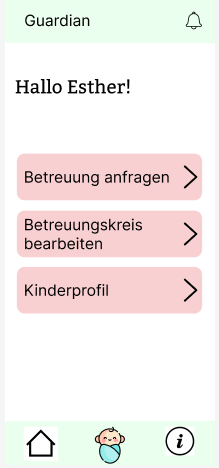
\includegraphics[width=0.2\linewidth]{media/Eltern-Startseite-1.draft.png}
    \caption{Startseite - Elternprofil (1. Draft)}
    \label{fig:1.Draft:Eltern:Startseite}
\end{figure}

% ---------------------------------------------------------------
% ------------- BEGIN TABLE -------------------------------------
% ---------------------------------------------------------------
\newpage
\textbf{1. Skizze - Funktionale Inhalte}
% Please add the following required packages to your document preamble:
% \usepackage{tabularx}
\begin{table}[h]
\centering
\begin{tabularx}{\linewidth}{|l|X|X|X|}
\hline
    & Startseite  & Betreuungsseite  & Profil  \\ \hline
                 
Eltern
& - Appname\newline - Notification-Symbol\newline - 3-4 Buttons = Shortcuts zu:\newline $\rightarrow$  Betreuungsanfrage stellen\newline $\rightarrow$ Betreuungskreis bearbeiten\newline $\rightarrow$ Kinder-Informationen bearbeiten
& Aktive Anfrage:\newline - Wer soll die Betreuung übernehmen\newline $\rightarrow$ vertraute Person oder Betreuungsagentur wählen\newline - Betreuungsdetails bearbeiten (Wann, Abholung, Betreuungsort, Gesundheit, Zusätzliche Hinweise)
& - hier: Kinderprofil\newline - Bearbeiten-Knopf einfügen\newline - allgmein: Name, Altern, Bild\newline - medizinische Informationen: Medikamente, Ärute / Hausarzt\newline - Kontakt: Adresse, Notfallkontakt (Telefonnummern) der der Eltern\newline - Einstellungen (Benachrichtigung, Datenschutz)                                                                                                         \\ \hline

Betreuungsperson
& - Appname\newline - Notification-Symbol\newline - Hallo {[}Name{]}\newline - 3-4 Buttons\newline $\rightarrow$ Neue Anfragen\newline $\rightarrow$ Betreuungskreise (Familien, die dich eingeladen haben)\newline $\rightarrow$ Mein Profil
& Anfrage:\newline - Status: Neu, Angenommen, Offen, Vergangen / Abgeschlossen\newline - Betreuungsdetails einsehen (Kindsname, Wann, Abholung, Betreuungsort, Gesundheit, Wichtige Hinweise)\newline - Button - Betreuung zusagen / Ablehnen
& - hier: Profil der BP\newline - Bearbeitenknopf einfügen\newline - Meine Verfügbarkeit (Zeiten festlegen)\newline - angebotene Dienstleistungen\newline $\rightarrow$ aus denen Eltern die zugetrauten Berechtigungen ableiten / auswählen können\newline $\rightarrow$  z.B. Betreuung bei sich oder bei Eltern, Abholen ja/nein, Arztbesuche ja/nein etc.\newline - Einstellungen (Benachrichtigung, Datenschutz)\\ \hline
\end{tabularx}
\end{table}
% ---------------------------------------------------------------
% ------------- END TABLE ---------------------------------------
% ---------------------------------------------------------------


% ***************************************************************
%           Ideate
% ***************************************************************
\subsection{Ideate}
\emph{Include Activity of Ideation Process.}

% ***************************************************************
%           Critical Reflection
% ***************************************************************
\subsection{Critical Reflection on Design Thinking}

\begin{itemize}
    \item What worked well with this approach for your project?
    \item What challenges did you encounter? (time constraints, participant recruitment, conflicting feedback)
    \item When did design thinking not provide clear direction?
    \item What alternative approaches might have been more effective?
\end{itemize}